\section{整体架构}

NApp Store整体上分为三个部分,Nebulas公链、NApp Store Client,NApp dev tools。Nebulas公链做为基础设施,已经开发完成,不在本文的描述范围内。NApp Store Client做为客户端,安装在每个用户的计算设备上,由用户直接使用。
NApp dev tools仅由开发者使用,是开发NApp所必要的生产工具。

概括来说,开发者使用NApp dev tools开发具有一定功能的NApp,并将生成的NApp提交到Nebulas公链之上。NApp Store Client通过同步最新的区块,得到开发者开发的NApp,并将该NApp对应的信息展示给用户。
最后,用户在NApp Store Client中选择想要执行的NApp,并执行相应的NApp。

开发者提交的NApp以LLVM IR的形式上链。开发者可以使用任意的、能编译生成LLRM IR的语言开发相应的NApp,通过NApp dev tools编译生成相应的LLVM IR,并最终通过NApp dev tools将LLVM IR提交上链。

NApp Store Client接入Nebulas公链的P2P网络,实时同步Nebulas公链中的区块,进行必要的区块信息验证,提取区块中的IR,并通过UI展示给用户。
在用户通过NApp的相关信息,选择想要执行的NApp之后,NApp Store Client将用户选中的IR与必要的库链接生成本地化的可执行应用,并执行。

\begin{figure}[ht!]
\centering
  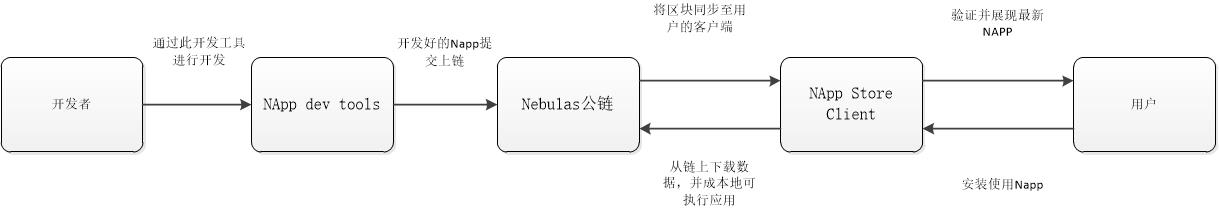
\includegraphics[width=.9\textwidth]{flow.jpg}
\caption{NApp Store 流程图}
\end{figure}

\subsection{NApp在链上的数据格式}
此处,我们给出NApp在链上的数据格式,以表明开发者需要提交哪些信息,并为后续的NApp Store Client的展示提供必要的数据。

我们使用protobuf的格式描述链上的数据结构。
\begin{verbatim}
message napp_dep_meta{
    string name = 1;
    uint64 version = 2;
};

message napp_data{
    string napp_name = 1;
    uint64 napp_version = 2;
    string napp_intro = 3;
    string napp_icon_url = 4;
    repeated napp_dep_meta napp_depends = 5;
    bytes napp_ir = 6;
};

\end{verbatim}
\noindent 其中,\texttt{napp\_name},\texttt{napp\_version},\texttt{napp\_intro},\texttt{napp\_icon\_url}的含义是明显的,需要注意的是\texttt{napp\_name}及\texttt{napp\_intro}皆有一定的长度限制。
\texttt{napp\_depends}定义了该NApp所依赖的库及版本号,\texttt{napp\_ir}为该NApp对应的LLVM IR。

另外,需要注意的是,由于一个transaction附带的binary data的长度通常有大小限制,因此,\texttt{napp\_data}的总长度不能超过对应的上限。目前,Nebulas主网对这一限制为128KB,这一限制可以进一步放松或解除。

\subsection{NApp能做什么?}
NApp并不是简单的智能合约或者简单的与智能合约的交互,NApp的能力很大程度上由其所依赖的库决定。最基础的部分,是一个NApp具有本地的与NAS账户、Nebulas主网及Nebulas主网之上的智能合约交互的能力;
更进一步的,NApp能够使用图形界面与用户进行交互、能够使用引擎创造更加本地化的应用体验。

举个例子,用户可以在NApp Store Client内安装一个书籍NApp,并在书籍NApp内完成支付、阅读、甚至评价等操作。
需要注意的是,其中的支付环节使用了书籍NApp与Nebulas交互的能力,阅读则使用了本地化的图形界面,最后的评价操作甚至涉及中心化的社交网络交互操作。
从这个例子中不难看出,NApp能够在使用区块链方面创造出流畅的用户体验。这将完全不同于现有的DApp需要使用额外的钱包或钱包插件的用户体验。

另外,从开发者的角度来看,开发NApp仅需要考虑本地化的开发及用户体验。这也有别于传统的DApp的开发,在DApp的开发中,由于智能合约不能提供本地化的交互体验,
因此,开发者需要通过前端(移动客户端或网页客户端)与智能合约进行交互,更复杂的,前端需要通过开发者自己架设的中心化服务器与区块链进行交互,这很大程度上增加了开发者的负担,同时也影响了用户体验。

\subsection{NApp与DApp的区别}
从概念上来说,NApp与DApp都包含了区块链交互的部分及用户交互的部分,其中区块链交互的部分通过智能合约,而在其他部分,这两者并不尽相同。

对于一个DApp,一般通过Web,或本地的客户端向用户提供交互接口,而Web或相应的客户端通过外部的钱包软件或插件与区块链进行交互,在一些情况下,Web或相应的客户端也可以通过中心化的服务器与区块链进行交互。
此时,由于缺乏统一的与区块链交互的方式,使得DApp在使用过程中,需要依赖外部的钱包软件或插件;更进一步地,Web、不同客户端之间的差异也使得区块链的使用难以有一致的开发或使用体验。

NApp则基于NApp dev tools包含的SDK与区块链进行交互,并使用其中的SDK构建图形化的用户交互界面,而进一步的流程及细节则由SDK提供保证,既保证了开发的简易性,又提供了体验的一致性。

另外,相对于DApp,NApp的一个重要能力是能够以去中心化的方式完成自动升级。对于使用了Web的DApp,可以通过在服务器中部署新的代码,而对于使用了客户端的用户,则依赖于用户的主动升级。

